\documentclass{article}

% if you need to pass options to natbib, use, e.g.:
% \PassOptionsToPackage{numbers, compress}{natbib}
\PassOptionsToPackage{square,numbers}{natbib}
\bibliographystyle{abbrvnat}
% before loading nips_2016
%
% to avoid loading the natbib package, add option nonatbib:
% \usepackage[nonatbib]{nips_2016}

% \usepackage{nips_2016}

% to compile a camera-ready version, add the [final] option, e.g.:
\usepackage[final]{nips_2016}

\usepackage{enumitem}
\usepackage[utf8]{inputenc} % allow utf-8 input
\usepackage[T1]{fontenc}    % use 8-bit T1 fonts
\usepackage[hidelinks]{hyperref}       % hyperlinks
\usepackage{url}            % simple URL typesetting
\usepackage{booktabs}       % professional-quality tables
\usepackage{amsfonts}       % blackboard math symbols
\usepackage{nicefrac}       % compact symbols for 1/2, etc.
\usepackage{microtype}      % microtypography

\usepackage{placeins}
\usepackage{float}
\usepackage{graphicx}
\usepackage{color}
\usepackage{mmstyles}
\DeclareGraphicsExtensions{.pdf,.png,.jpg,.eps}

\newcommand{\misscite}{\textcolor{red}{[CITE]}}
\newcommand{\missref}{\textcolor{red}{R}}
\newcommand{\real}{{\mathbb{R}}}
\newcommand{\zz}{{\mathbb{Z}}}
\newcommand{\bt}{{\mathbf{t}}}
\newcommand{\bx}{{\mathbf{x}}}
\newcommand{\by}{{\mathbf{y}}}
\newcommand{\bu}{{\mathbf{u}}}
\newcommand{\bg}{{\mathbf{g}}}
\newcommand{\bh}{{\mathbf{h}}}
\newcommand{\bR}{{\mathbf{R}}}

\title{ELEG 5491 HW2}

% The \author macro works with any number of authors. There are two
% commands used to separate the names and addresses of multiple
% authors: \And and \AND.
%
% Using \And between authors leaves it to LaTeX to determine where to
% break the lines. Using \AND forces a line break at that point. So,
% if LaTeX puts 3 of 4 authors names on the first line, and the last
% on the second line, try using \AND instead of \And before the third
% author name.

\author{
	Zhizhong Li \\
	\emph{Mar 2017} \\
	Information Engineering, CUHK\\
	\texttt{1155070507, lz015@ie.cuhk.edu.hk} \\
}

\begin{document}
	% \nipsfinalcopy is no longer used

\maketitle

\section{Problem 1}~\label{sec:prob1}

\subsection{} % 1.1

Under the conditions specified in the problem,
we cannot arrive at that conclusion.
Here is an counter example.
Let $m=n=r$, then $U=V=\real^n$.
So $\M=\Mbar=\real^{n\times n}$.

To make this question more sensible,
let us impose an extra condition that
$r<\min(m,n)=m$.
First the fact that $\M \subset \Mbar$ is trivial to verify
($\forall X \in \M$ and $\forall Y \in \Mbar^\perp$, $X\cdot Y=0$,
so $\M \subset (\Mbar^\perp)^\perp=\Mbar$).
We focus on why it is a proper subset.

Construct two orthogonal matrices $P\in\real^{m\times r}$,
and $Q\in \real^{r\times n}$, s.t.,
$\col(P)=U$ and $\row(Q)=V$.
Then $\forall X\in\M$, it can be decomposed as
$X=P\Sigma Q$, where $\Sigma\in\real^{r\times r}$
(This is fairly easy to see after an svd on X).
The decomposition is unique.
For two decompositions of $X$,
say $X=P\Sigma_1 Q=P\Sigma_2 Q$,
then multiply $P^T$ and $Q^T$ at the left and right hand of the equation,
we have $\Sigma_1=\Sigma_2$.
So we get an one-to-one mapping from $\M$ to $\real^{r\times r}$.
This mapping is also linear (easy to verify).
Thus $\dim \M \le \dim \real^{r\times r} = r^2$.
Similar story goes to $\Mbar^\perp$ and we have
$\dim \Mbar^\perp \le \dim \real^{(m-r)\times(n-r)} = (m-r)(n-r)$.
Thus $\dim \M + \dim \Mbar^\perp \le r^2 + (m-r)(n-r) < mn = \dim \real^{m\times n}$.
This is a contradiction if $\M=\Mbar$ because
the sum of $\dim \Mbar(=\dim \M)$ and $\dim \Mbar^\perp$ should be $mn$ then.

\subsection{} % 1.2

Let orthogonal matrices $P=(P_1\ P_2)\in\real^{m\times m}$ and
$Q=(Q_1^T\ Q_2^T)^T\in\real^{n\times n}$, s.t.
$\col(P_1)=U, \col(P_1) = U^\perp, \row(Q_1) = V, \row(Q_2)=V^\perp$.
Then similar to the last sub-question,
$\forall X\in\M, \forall Y\in\Mbar^\perp$,
we can decompose them as
\begin{equation}
    X =
        \begin{bmatrix}
        P_1 & 0\\
        \end{bmatrix}
        \begin{bmatrix}
        \Sigma_1 &   0 \\
        0 & 0\\
        \end{bmatrix}
        \begin{bmatrix}
        Q_1 \\
        0 \\
        \end{bmatrix},\quad
        Y =
        \begin{bmatrix}
        0 & P_2\\
        \end{bmatrix}
        \begin{bmatrix}
        0 &   0 \\
        0 & \Sigma_2\\
        \end{bmatrix}
        \begin{bmatrix}
        0 \\
        Q_2 \\
        \end{bmatrix},
\end{equation}
where $\Sigma_1\in\real^{r\times r}$ and $\Sigma_2\in\real^{(m-r)\times(n-r)}$.
So,
\begin{equation}
    X + Y =
        \begin{bmatrix}
        P_1 & P_2\\
        \end{bmatrix}
        \begin{bmatrix}
        \Sigma_1 &   0 \\
        0 & \Sigma_2\\
        \end{bmatrix}
        \begin{bmatrix}
        Q_1 \\
        Q_2 \\
        \end{bmatrix}.
\end{equation}
Thus,
$\|X+Y\|_*=\|\Sigma_1+\Sigma_2\|_*=\|\Sigma_1\|_*+\|\Sigma_2\|_*=\|X\|_*+\|Y\|_*$.


\section{Problem 2}~\label{sec:prob2}

\subsection{} % 2.1

Since $(\E[\|g\|_2])^2 \le \E[\|g\|_2^2]$,
and $\|g\|_2^2$ follows a chi-square distribution,
we have $\E[\|g\|_2^2]=n$,
and thus $\E[\|g\|_2]\le \sqrt{n}$.

\subsection{} % 2.2

\begin{equation}
\begin{split}
\prob(\|g\|_2^2\le\alpha n) & = \prob(\exp(t(\alpha n-\|g\|_2^2))\ge 1) \\
    & \le  \E[\exp(t(\alpha n-\|g\|_2^2))]  \\
    & = \exp(t\alpha n) \E(\exp(-t\|g\|_2^2))   \\
    & = \exp(t\alpha n) (1+2t)^{-n/2}. \\
%     % & = \exp(t\alpha n) ()
\end{split}
\end{equation}

Note that the inequality comes from the Markov inequality and
the last equation is obtained by the moment-generating
function of a Chi-squared $\chi^2_n$ random variable
being $(1-2t)^{-n/2}$.

\subsection{} % 2.3

Let $t=(1-\alpha)/(2\alpha)$,
and from the inequality from last sub-question,
we have

\begin{equation}
    \prob(\|g\|_2^2\le\alpha n) \le \exp((1-\alpha + \ln \alpha)n/2).
\end{equation}


\section{Problem 3}

Since $h(\cA(X))$ is smooth,
we compute the derivative
\begin{equation}
    D:=\frac{\partial h(\cA(X))}{\partial X} =
    \begin{bmatrix}
        \frac{3}{2}X_{11}-2X_{22}-\frac{5}{2} & 0 \\
        0   & -2X_{11}+3X_{22}+1 \\
    \end{bmatrix}.
\end{equation}
The two numbers in the matrix come from
\begin{equation}
\begin{split}
    \frac{\partial h(y)}{\partial y}
        &= (B^{\frac{1}{2}})^T(B^{\frac{1}{2}}y-B^{-\frac{1}{2}}d) \\
        &= By-d.
\end{split}
\end{equation}

The optimality condition at point $X$ is
\begin{equation}
    0\in\{D+W:W\in\partial\|X\|_*\}.
\end{equation}
Or equivalently,
\begin{equation}\label{eq:cond}
    -D\in\partial\|X\|_*.
\end{equation}

For $X=0$,
$\partial\|X\|_*=\{W:\|W\|\le1\}$.
However,
$\|-D\|=2.5>1$.
So $X=0$ is not a solution.

If $X$ is rank 2,
suppose one of its SVD is $X=U\Sigma V^T$
and $\sigma_1\ge\sigma_2>0$.
Then $\partial\|X\|_*=UV^T$.
We get the constraint
\begin{equation}
    -D=UV^T.
\end{equation}
The right hand side can be seen as an SVD of $-D$
with $\sigma_1(D)=\sigma_2(D)=1$.
Since $D$ is a diagonal matrix,
we have
\begin{equation}
\begin{split}
    \frac{3}{2}X_{11}-2X_{22}-\frac{5}{2} &= \pm1, \\
    -2X_{11}+3X_{22}+1 &= \pm1.
\end{split}
\end{equation}


\section{Problem 4}~\label{sec:prob4}

\subsection{} % 4.1

\begin{equation}
\begin{split}
[[L_\bt f] * w](\bx)
    & = \sum_{\by\in \zz^2}\sum_{k=1}^K (L_\bt f_k)(\by) w_k(\by-\bx)  \\
    & = \sum_{\by\in \zz^2}\sum_{k=1}^K f_k(\by-\bt) w_k(\by-\bx)  \\
    & = \sum_{\by\in \zz^2}\sum_{k=1}^K f_k(\by) w_k(\by-(\bx-\bt))  \\
    & = [ f * w](\bx-\bt) \\
    & = [L_\bt[ f * w]](\bx).
\end{split}
\end{equation}

\subsection{} % 4.2

\begin{equation}
\begin{split}
[[L_\bR f] * w](\bx)
    & = \sum_{\by\in \zz^2}\sum_{k=1}^K (L_\bR f_k)(\by) w_k(\by-\bx)  \\
    & = \sum_{\by\in \zz^2}\sum_{k=1}^K f_k(\bR^{-1} \by) w_k(\by-\bx)  \\
    & = \sum_{\by\in \zz^2}\sum_{k=1}^K f_k(\by) w_k(\bR\by-\bx))  \\
    & = \sum_{\by\in \zz^2}\sum_{k=1}^K f_k(\by) w_k(\bR(\by-\bR^{-1} \bx))  \\
    & = \sum_{\by\in \zz^2}\sum_{k=1}^K f_k(\by) [L_{\bR^{-1}} w_k](\by-\bR^{-1} \bx)  \\
    & = [ f *  [L_{\bR^{-1}} w]](\bR^{-1} \bx) \\
    & = [L_\bR[ f * [L_{\bR^{-1}} w]]](\bx).
\end{split}
\end{equation}

\subsection{} % 4.3


\section{Problem 5}~\label{sec:prob5}

\subsection{} % 5.1

The training curve is shown in Figure~\ref{fig:1}.
The learned filters is shown in Figure~\ref{fig:2}.
Comparison between weight decay and no weight decay is shown in Figure~\ref{fig:3}.

\begin{figure}[ht]
\centering
    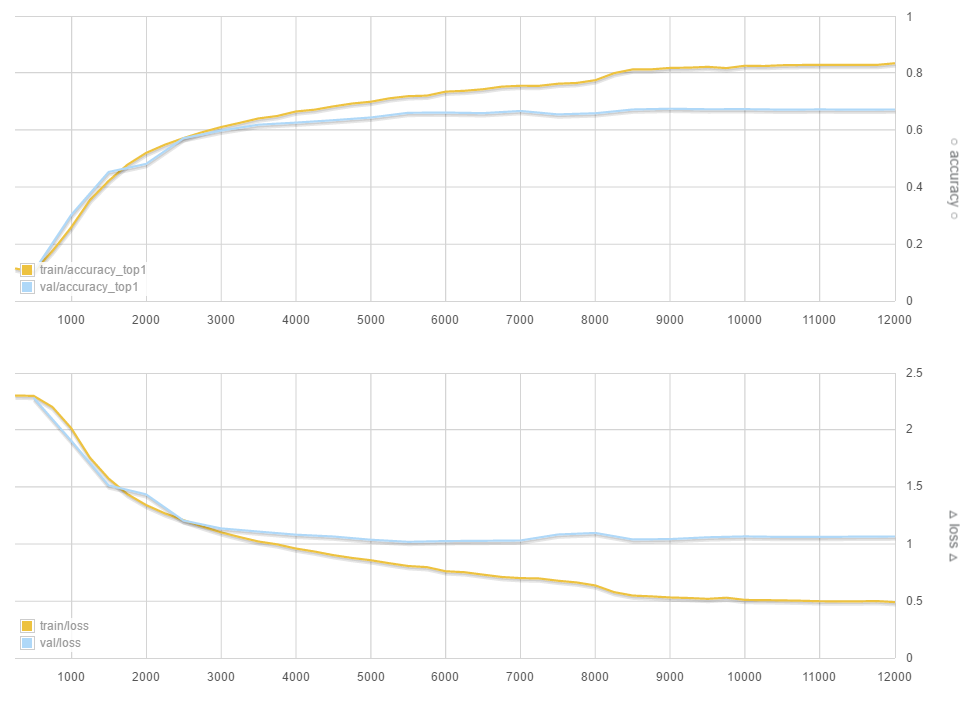
\includegraphics[width=0.99\linewidth]{fig/curve1}
    \caption{\small
    Training curve of the simple network on CIFAR-10.
    initialization is Gaussian.
    The batch size is 256.
    Use SGD as described in the problem.
    The step sizes are 8000, 10000 and 12000.}
    \label{fig:1}
\end{figure}

\begin{figure}[ht]
\centering
    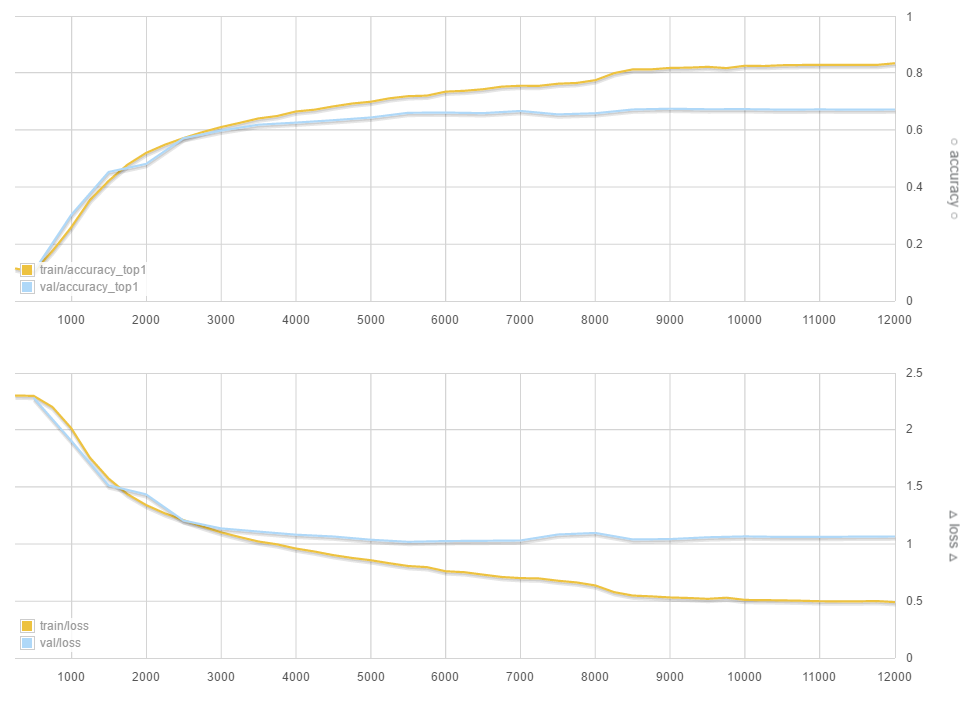
\includegraphics[width=0.99\linewidth]{fig/curve1}
    \caption{\small
    Filters of the first convolutional layer.}
    \label{fig:2}
\end{figure}

\begin{figure}[ht]
\centering
    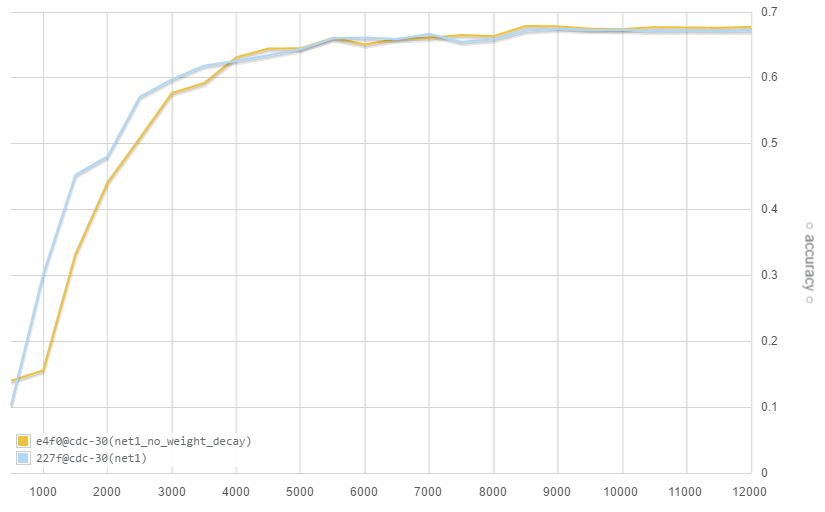
\includegraphics[width=0.9\linewidth]{fig/nodecayacc}
    \caption{\small
    With or without weight decay.
    We can see that they do not have significant difference.
    The one with weight decay has best val accuracy $67.44\%$.
    The one without weight decay has best val accuracy $67.86\%$.}
    \label{fig:3}
\end{figure}


\subsection{} % 5.2

Since $w_l$ has zero mean,
so does $w_l x_l$.
Together with independence between $x_l$ and $w_l$,
we have

\begin{equation}
\begin{split}
    \Var[y_l] &= n_l \Var[w_l x_l] \\
        &=n_l E[w_l^2 x_l^2] - 0 \\
        &=n_l E[w_l^2] E[x_l^2] \\
        &=n_l \Var[w_l] E[x_l^2].
\end{split}
\end{equation}

To prove $E[x_l^2]=Var[y_{l-1}]/2$,
we need assume that $y_{l-1}$ is Gaussian with zero mean.
Since
\begin{equation}
    x_l = \begin{cases}
        y_l, &\text{ if }y_l\ge0\\
        0, , &\text{ if }y_l<0\\
    \end{cases}
\end{equation}
So
\begin{equation}
    E[x_l^2] = \int_0^\infty p(x_l)x_l^2 dx_l
        = \frac{1}{2}\int_{-\infty}^\infty p(x_l)x_l^2 dx_l
        = \frac{1}{2}Var[y_{l-1}].
\end{equation}

The initialization described here is the \emph{msra} initialization~\cite{he2015delving}.

\subsection{} % 5.3

\subsection{} % 5.4


\medskip

\bibliography{bf}


\end{document}
